Pour créer une nouvelle partie, appuyez sur le bouton \emph{Nouvelle partie} au lancement du jeu ou allez dans le menu \emph{Fichier} -> \emph{Nouvelle partie} (attention, tous les changements non sauvegardés sur votre partie en cours seront alors perdus).
Ensuite, une boîte de dialogue s'affiche, vous demandant de choisir les options de la partie :

\begin{figure}[!h]
\centering
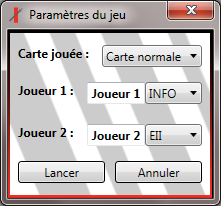
\includegraphics{Parties/Images/CreationPartie.png}
\caption{La fenêtre de création de partie}
\label{fig:CreationPartie}
\end{figure}

\begin{description}
	\item[Carte jouée :] le type de carte désiré, voir partie \ref{sec:typesJeu}.

	\item[Nom du joueur :] le nom de chaque joueur. Les noms ne peuvent être identiques.

	\item[Département du joueur :] le département que chaque joueur souhaite incarner. Il est possible pour deux joueur de choisir le même département.
\end{description}

Une fois ces options choisies, cliquez sur \emph{Lancer} pour lancer la partie, ou sur \emph{Annuler} pour annuler la partie.